\taskpic{ На нижнюю поверхность горизонтальной диэлектрической
  пластины толщиной $d$ с диэлектрической проницаемостью $\eps$
  нанесено проводящее покрытие. На верхнюю поверхность помещена
  маленькая капля ртути, которая не смачивает пластину. Капля и
  проводящее покрытие образуют конденсатор. При каком напряжении
  батареи капля начнёт растекаться по поверхности пластины?
  Коэффициент поверхностного натяжения ртути $\sigma$. }
{
  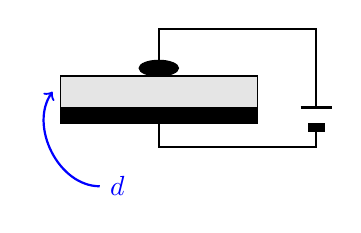
\begin{tikzpicture}
    \draw[fill=gray!20] (0,0) rectangle (2.5,0.4) node[midway] {$\eps$};
    \draw[fill=black] (0,0) rectangle (2.5,-0.2);
    \draw[fill=black] (1.25,0.5) ellipse (0.25cm and 0.1cm);
    \draw[thick] (1.25,0.5) -- (1.25,1) -- (3.25,1) -- (3.25,0cm);
    \draw[thick] (3.25,-0.3cm) -- (3.25,-0.5cm) -- (1.25,-0.5cm) --
    (1.25,-0.2cm);
    \draw[fill=black] (3.15,-0.3cm) rectangle (3.35,-0.2cm);
    \draw[thick] (3.05,0) -- (3.45,0);
    \draw[blue,thick,->] (0.5,-1) node[right] {$d$}
    to[out=180,in=235] (-0.1,0.2cm); 
  \end{tikzpicture}
}
% Москва, город-1992, 10 класс